\documentclass[11  pt]{article} 
\usepackage[lmargin=1in,rmargin=1.75in,bmargin=1in,tmargin=1in]{geometry}  


% For hyperlinking everything
\usepackage{hyperref}
\hypersetup{
	colorlinks=true, %set true if you want colored links
	linktoc=all,     %set to all if you want both sections and subsections linked
	linkcolor=blue,  %choose some color if you want links to stand out
}


\usepackage[latin1]{inputenc}
\usepackage{amsmath}
\usepackage{mathrsfs}  
\usepackage{amsfonts}
\usepackage{amssymb}
\usepackage{graphicx}
\usepackage{subfig}
\usepackage{caption}
\usepackage{algorithm}
%\usepackage{algcompatible}
%\usepackage{algorithmicx}
\usepackage{algpseudocode}

\usepackage{titlesec}
\titleformat{\section}{\fontfamily{lmss}\fontsize{14}{15}\bfseries}{\thesection}{1em}{}
\titleformat{\subsection}{\fontfamily{lmss}\fontsize{12}{15}\bfseries}{\thesubsection}{1em}{}




\usepackage{amsthm}

\newtheoremstyle{noit}
{10pt}% <Space above>
{10pt}% <Space below>
{}% <Body font>
{}% <Indent amount>
{\bfseries}% <Theorem head font>
{.}% <Punctuation after theorem head>
{.5em}% <Space after theorem headi>
{}% <Theorem head spec (can be left empty, meaning `normal')>

\newtheoremstyle{example}
{10pt}% <Space above>
{10pt}% <Space below>
{}% <Body font>
{20pt}% <Indent amount>
{\bfseries}% <Theorem head font>
{.}% <Punctuation after theorem head>
{.5em}% <Space after theorem headi>
{}% <Theorem head spec (can be left empty, meaning `normal')>


\newtheoremstyle{indented}{20pt}{20pt}{\addtolength{\leftskip}{2.5em}}{}{\bfseries}{.}{.5em}{}


\newtheorem{theorem}{Theorem}
\numberwithin{theorem}{section}
\newtheorem{lemma}[theorem]{Lemma}
\newtheorem{corollary}[theorem]{Corollary}
\newtheorem{observation}{Observation}
%\numberwithin{observation}{section}
%\numberwithin{definition}{section}
\newtheorem{conjecture}{Conjecture}
\newtheorem{Qu}{Question}
\newcommand{\QU}{\begin{Qu}\normalfont}

\theoremstyle{noit}
\newtheorem{fact}{Fact}
\newtheorem{definition}{Definition}

\theoremstyle{indented}
\newtheorem{example}{Example}

\theoremstyle{indented}
\newtheorem{problem}{Problem}


%\newenvironment{proof}{\noindent{\bf Proof:} \hspace*{1em}}{
%    \hspace*{\fill} $\Box$ }
%\newenvironment{proof_of}[1]{\noindent {\bf Proof of #1:}
%    \hspace*{1em} }{\hspace*{\fill} $\Box$ }
%\newenvironment{proof_claim}{\begin{quotation} \noindent}{
%    \hspace*{\fill} $\diamond$ \end{quotation}}
\newcommand{\vs}[1]{\vspace{#1}}

\newcommand{\lecture}[2]{
 \noindent
\begin{center}
	\framebox{
		\vbox{
			\hbox to 5.78in { {\bf CSCE 411: Design and Analysis of Algorithms} \hfill  }
			\vspace{2mm}
			\hbox to 5.78in { {\Large \hfill Lecture #1\hfill} }
			\vspace{2mm}
			\hbox to 5.78in { {\it Date: #2 \hfill Lecturer: Nate Veldt} }
		}
	}
\end{center}
\vspace*{4mm}
}


\newcommand{\hw}[2]{
	\noindent
	\begin{center}
		\framebox{
			\vbox{
				\hbox to 5.78in { {\bf CSCE 411: Design and Analysis of Algorithms} \hfill  }
				\vspace{2mm}
				\hbox to 5.78in { {\Large \hfill Homework #1\hfill} }
				\vspace{2mm}
				\hbox to 5.78in { {\it Due date: #2 \hfil} }
			}
		}
	\end{center}
	\vspace*{4mm}
}



\newcommand{\under}[1]{\underline{\hspace{#1}}}
\setlength{\parindent}{0em}

%\usepackage[tagged]{accessibility}

% Graph terms
\newcommand{\vol}{\textbf{vol}}
\newcommand{\cut}{\textbf{cut}}


% Matrices
\newcommand{\mA}{\textbf{A}}
\newcommand{\mB}{\textbf{B}}

% vectors
\newcommand{\ve}{\textbf{e}}
\newcommand{\vx}{\textbf{x}}


% Other
\newcommand{\calN}{\mathcal{N}}

\usepackage{mathtools}
\DeclarePairedDelimiter\ceil{\lceil}{\rceil}
\DeclarePairedDelimiter\floor{\lfloor}{\rfloor}


\newcommand*{\aitem}{ \item[{
\includegraphics[width=0.8cm,height=0.5cm]{../../Lectures/figures/A}} ]  }
\newcommand*{\bitem}{ \item[{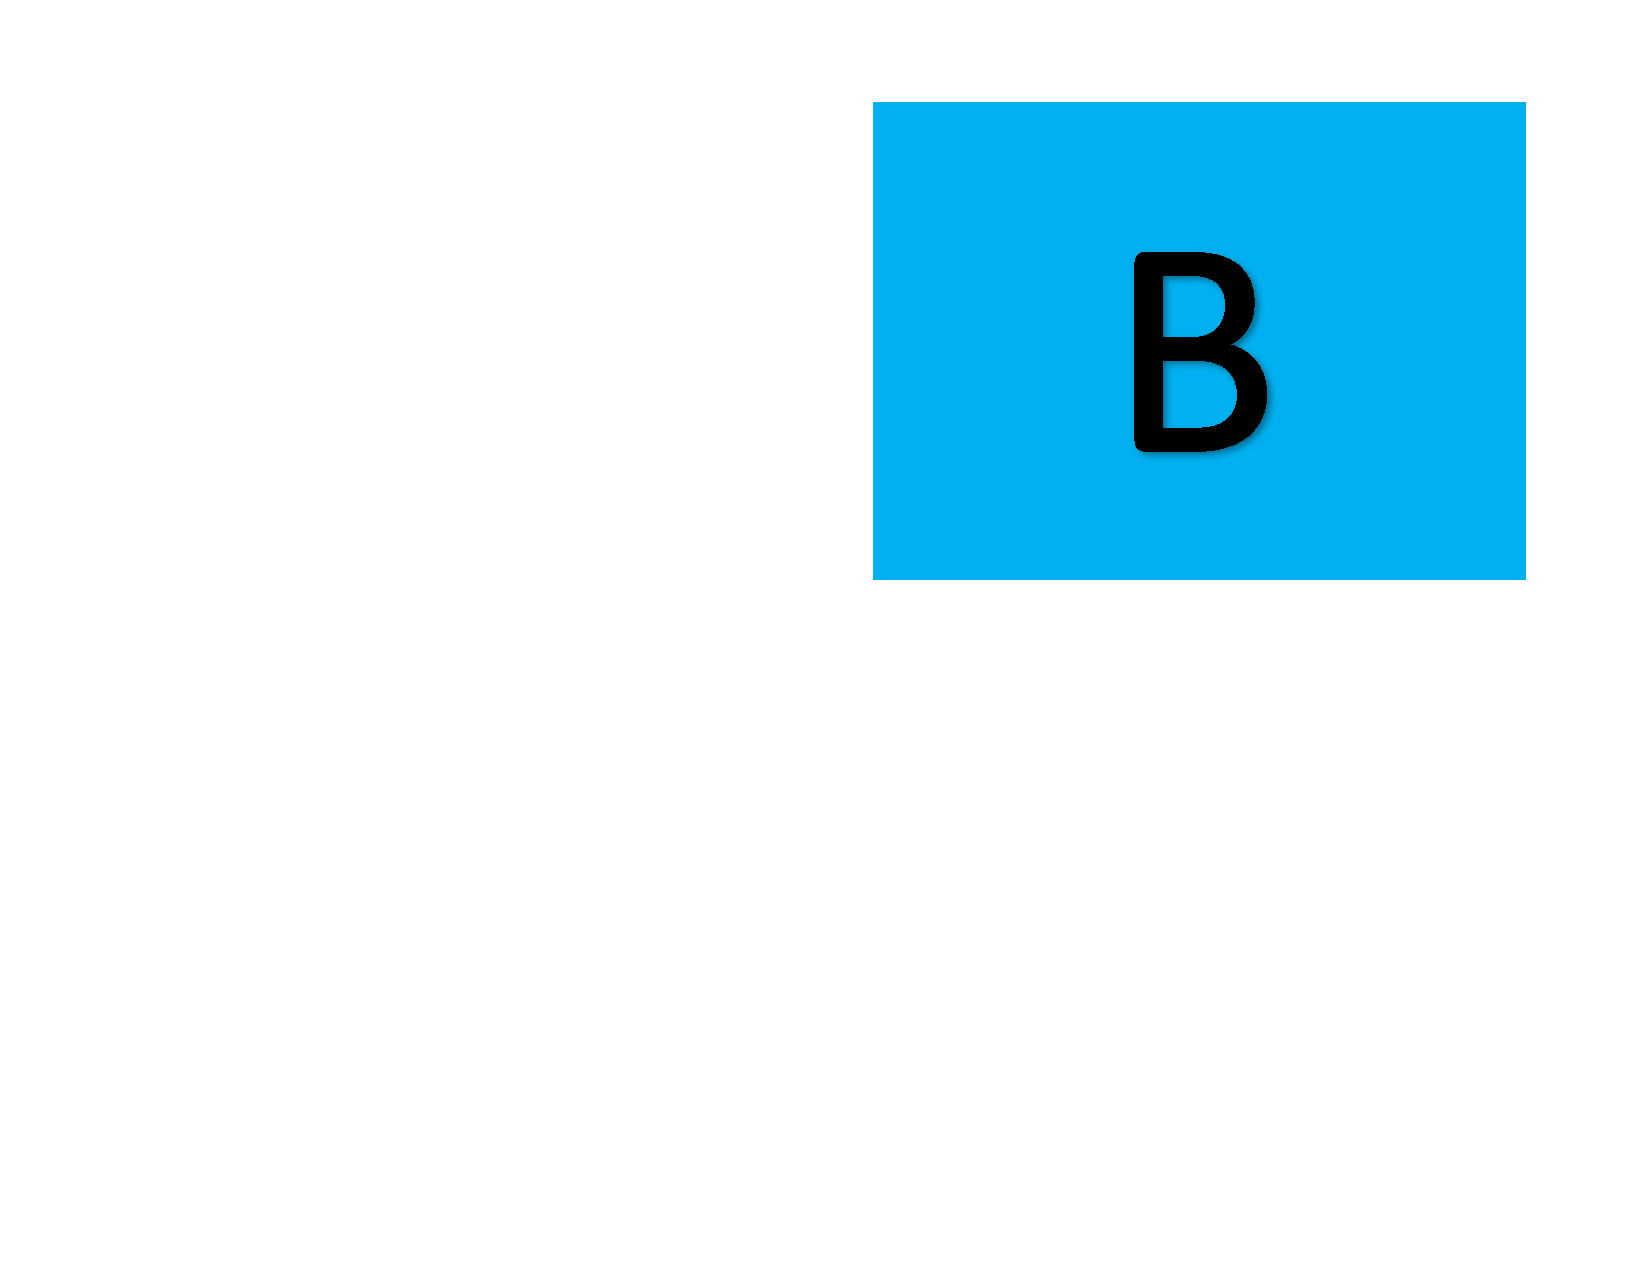
\includegraphics[width=0.8cm,height=0.5cm]{../../Lectures/figures/B}} ]  }
\newcommand*{\citem}{ \item[{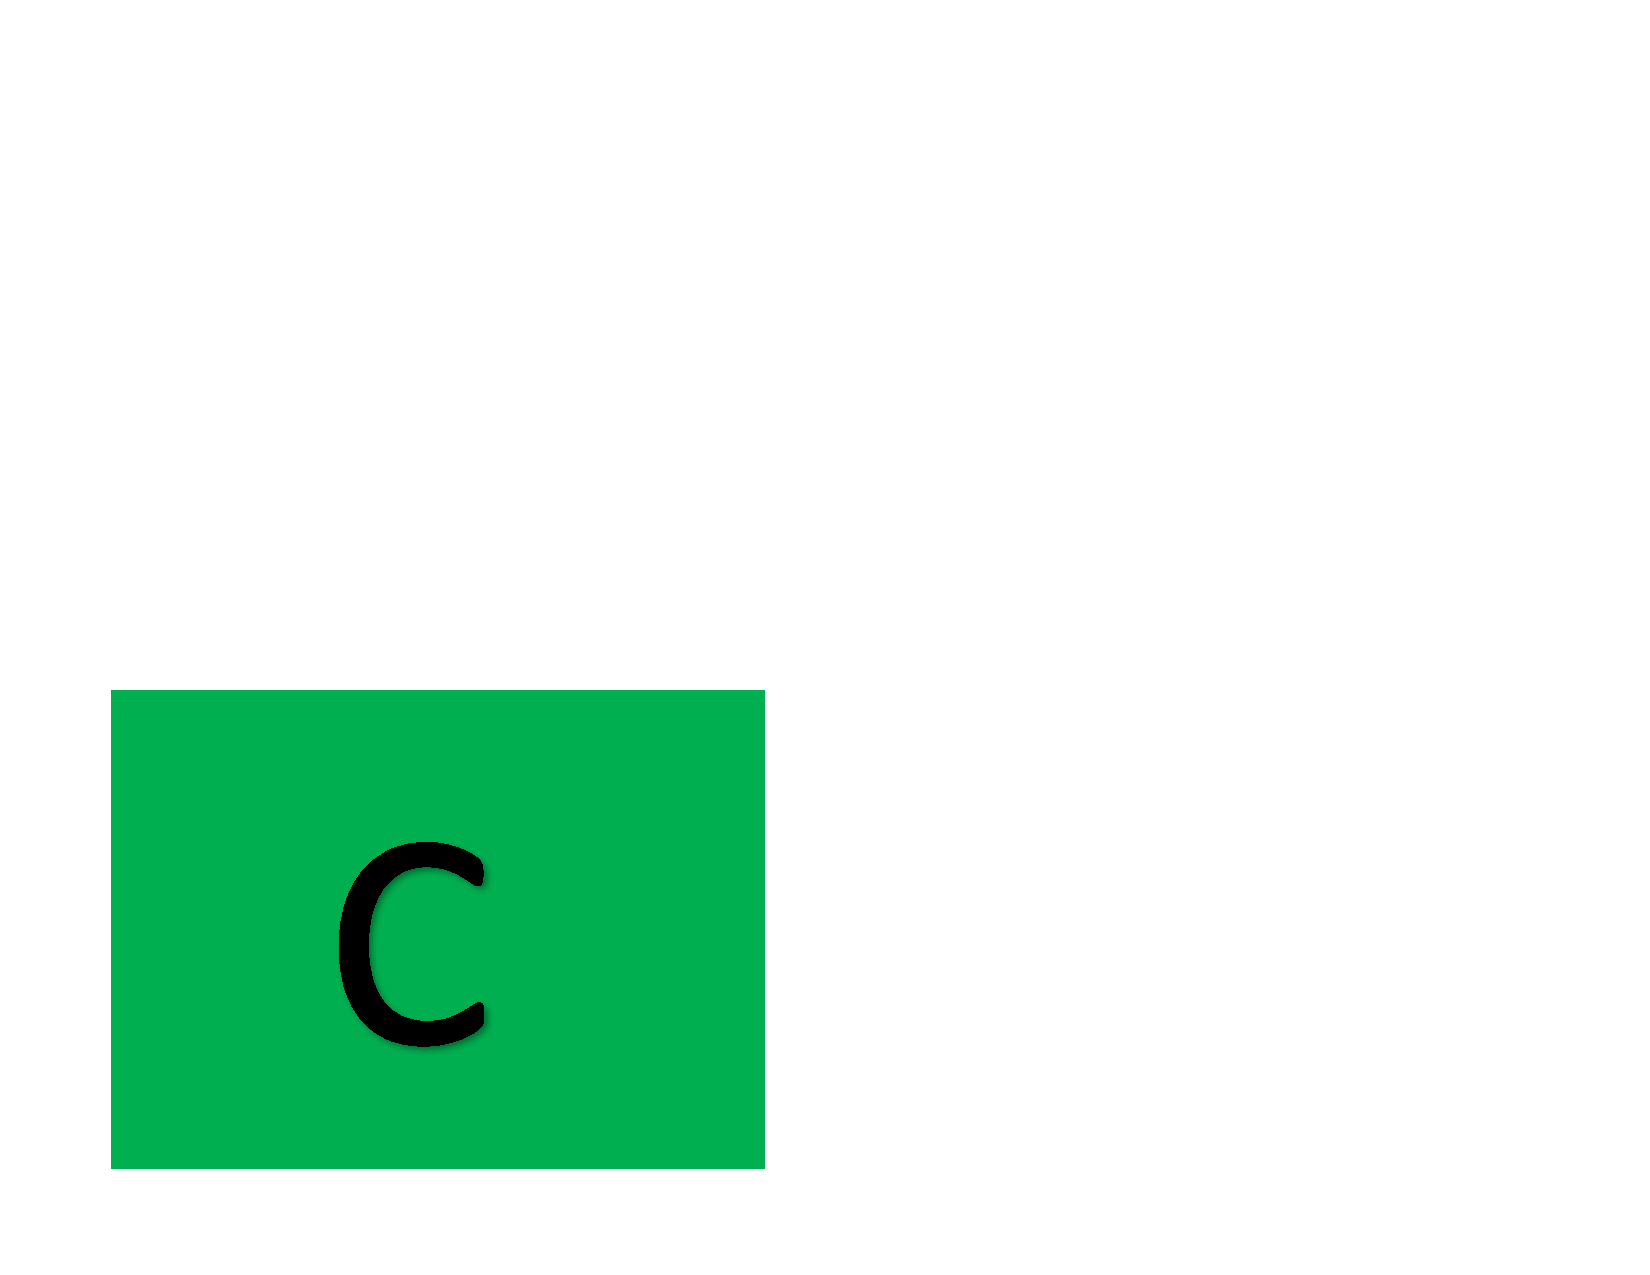
\includegraphics[width=0.8cm,height=0.5cm]{../../Lectures/figures/C}} ]  }
\newcommand*{\ditem}{ \item[{
\includegraphics[width=0.8cm,height=0.5cm]{../../Lectures/figures/D}} ]  }
\newcommand*{\eitem}{ \item[{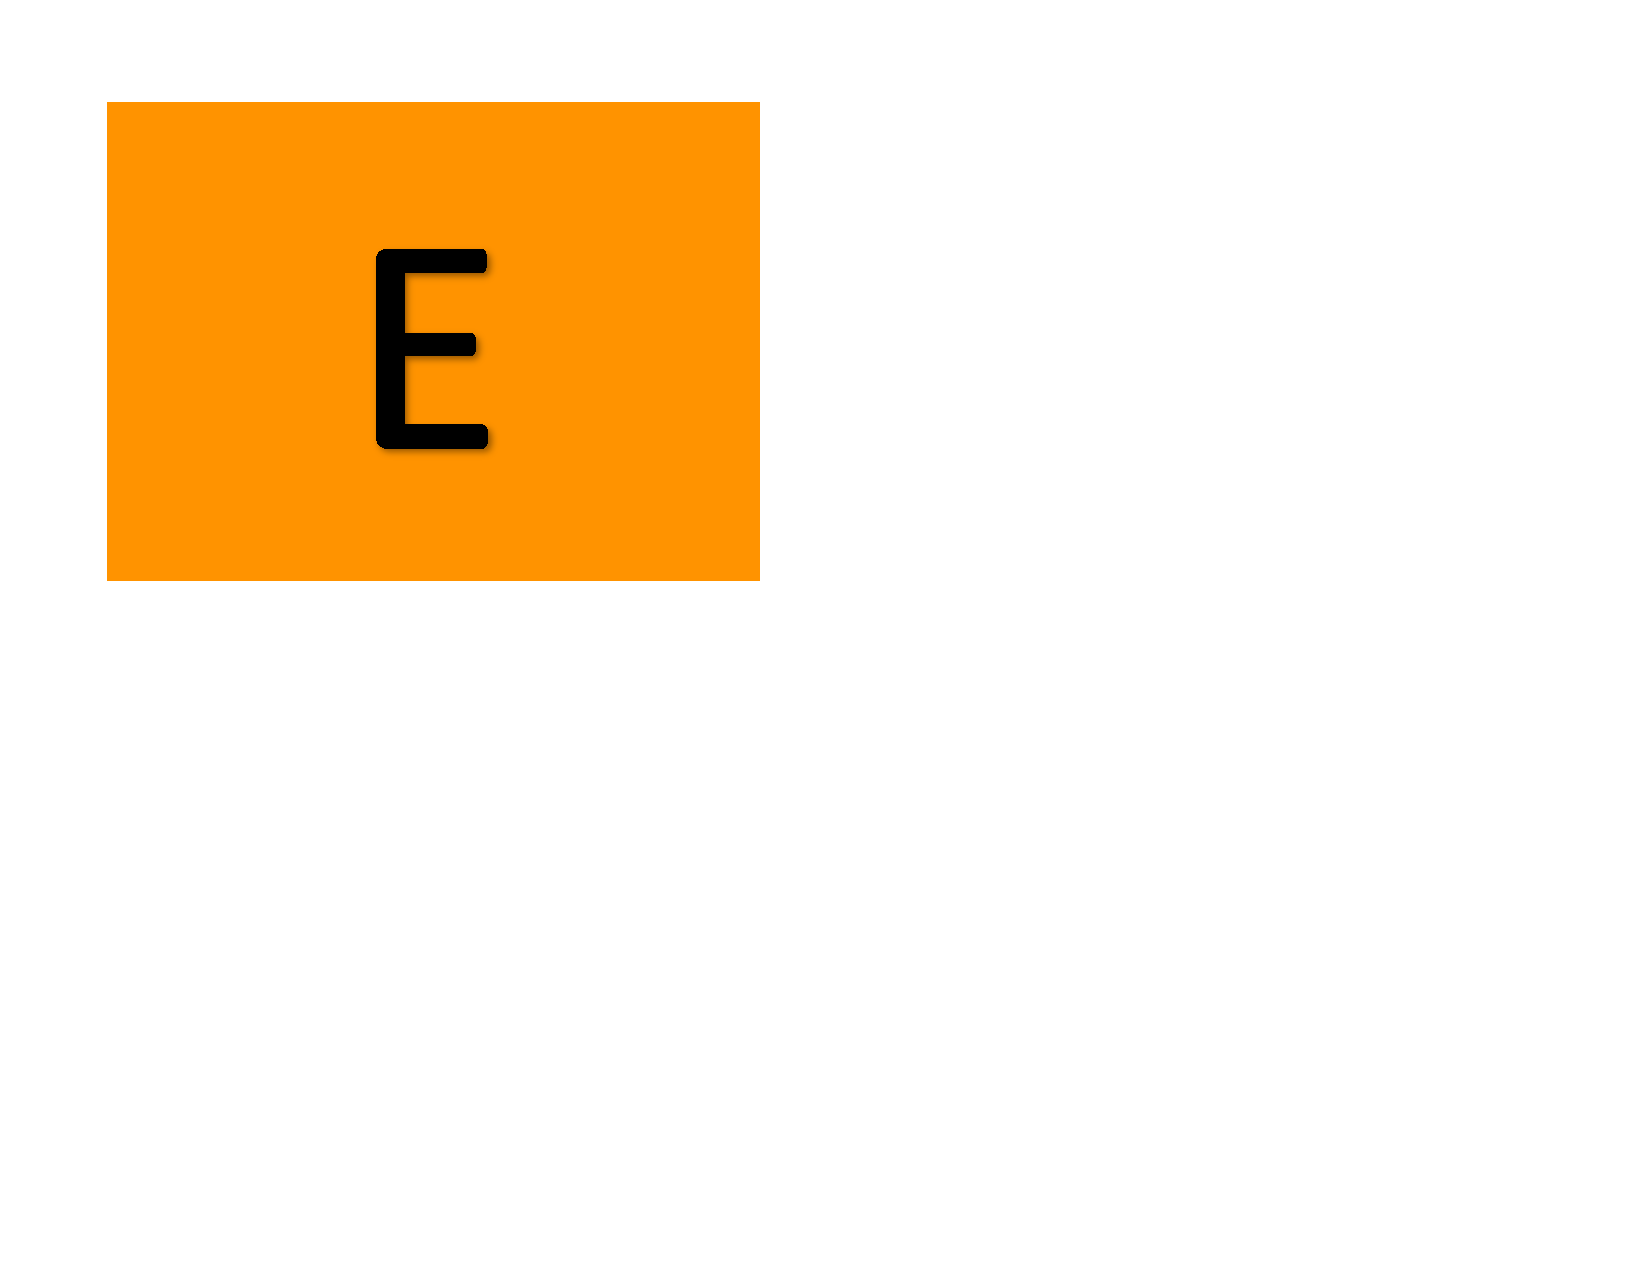
\includegraphics[width=0.8cm,height=0.5cm]{../../Lectures/figures/E}} ]  }
\newcommand*{\fitem}{ \item[{
\includegraphics[width=0.8cm,height=0.5cm]{../../Lectures/figures/F}} ]  }


\newcommand{\hide}[1]{\underline{\phantom{#1 #1}}}

\usepackage{setspace}

\onehalfspacing

\begin{document}
	
	\lecture{: Approximation Algorithms and Optimization}{Week 14}
	\textbf{Course Logistics}
	\begin{itemize}
		\item CLRS Chapter 34
		\item Homework due Friday
	\end{itemize}
	
	\section{Approximation Algorithms for Optimization Problems}
There are so many hard problems out there without known polynomial time solutions! Is all hope lost? What do we do?

\vs{1cm}
\textbf{Approximation algorithms} ``quickly'' find an answer that is ``close'' to the solution.

\vs{4cm}
We are now focused on optimization problems, rather than just their decision versions.

\vs{1cm}
\textbf{Definition.} Let $Q$ be a computational minimization problem (e.g., find a minimum vertex cover, find a minimum s-t cut) and assume that $C^*$ is the optimal (minimum) solution to the problem. An \hide{approximation algorithm} for $Q$ with approximation factor $p$ is an algorithm that:
\begin{itemize}
    \item Runs in 
    \item Outputs a solution value $C$ that is guaranteed to satisfy

\vs{4cm}
\end{itemize}

\QU
What is a lower bound we must assume holds for the value of $p$ when defining an approximation algorithm?
\begin{enumerate}
	\aitem No lower bound is needed, $p$ can be any real number.
	\bitem $p \geq -1$.
	\citem $p \geq 0$.
	\ditem $p \geq 1$.
	\eitem $p \geq C^*$.
\end{enumerate}
\end{Qu}

\vs{1cm}
We can also have approximation algorithms for maximization problems, but in this case $C^*$ represents the maximum value (i.e., the solution) for the problem and \hide{$p\le 1$}

\vs{1cm}
\textbf{Wait, is this even possible?} We want to guarantee that $\frac{C}{C^*}$ is small in polynomial time, but finding $C^*$ is NP-hard. How can we do that?

\vs{1cm}
To design an approximation algorithm, we need two pieces:

\begin{enumerate}
    \item \hide{Lower bound} A procedure for finding a value $\hat{C}$ that satisfies \hide{$\hat{C}\le C^*$}
    \begin{itemize}
        \item It should take polynomial time.
				
				\vs{0.5cm}
        \item This method \hide{does not} solve the original problem, but is often related.
    \end{itemize}
    \item \hide{Upper bound} An algorithm for the original problem that returns a suboptimal solution \hide{$C\ge C^*$}
    \begin{itemize}
        \item It should take polynomial time.
				
				\vs{0.5cm}
        \item This method often: %leverages $\hat{C}$ or problem structure.
    \end{itemize}
\end{enumerate}

We then must prove that \hide{$\frac{C}{C^*} \leq p$} and this provides a $p$-approximation!

\vs{4cm}
\textbf{Caveat.} Often, the lower bounding procedure is \emph{explicit}: there is an actual algorithm that computes the lower bound, and then the upper bounding algorithm explicitly uses the lower bound. However, in some cases no explicit lower bound is computed, and instead one shows implicitly that the upper bounding algorithm must provide a solution that is better than some lower bound, even though the lower bound isn't computed explicitly. This can be tricky, but it is often possible!


\section{Matchings and Vertex Covers}
Let $G = (V, E)$ be an undirected and unweighted graph.


\vs{1cm}
A \textbf{matching} $M \subseteq E$ is a set of edges such that no two edges share the same node.


\vs{1cm}
A \textbf{vertex cover} $C \subseteq V$ is a set of nodes such that each edge $(u, v) \in E$ has at least one node in $C$.

\vs{5cm}
\begin{lemma}
Let $M$ be a matching of $G$ and $C$ be a vertex cover. Then $|M| \leq |C|$.
\end{lemma}

\vfill

\section{The approximation algorithm for vertex cover}
A matching $M \subseteq E$ is a \textbf{maximal matching} if for every edge $e \in E \setminus M$, $M \cup \{e\}$ is no longer a matching.

\vs{8cm}
\textbf{The algorithm} \\
\texttt{VertexCoverApprox}($G = (V, E)$)
\begin{enumerate}
    \item Compute a maximal matching $M$ of $G$:
    \begin{itemize}
        \item Set $F = E$, $M = \emptyset$.
        \item While $|F| > 0$:
        \begin{itemize}
            \item Add any edge $e \in F$ to $M$.
            \item For each remaining $f \in F$, if $|e \cap f| > 0$, remove $f$ from $F$.
        \end{itemize}
    \end{itemize}
    \item Let $S$ be the set of nodes adjacent to an edge in $M$.
    \item Return $S$.
\end{enumerate}

\newpage
\begin{theorem}
Let $C^*$ be the minimum sized vertex cover of $G$. The algorithm \texttt{VertexCoverApprox} runs in polynomial time in terms of the size of $G$ and outputs a vertex cover $S \subseteq V$ satisfying $|S| \leq 2C^*$. Thus, this is a 2-approximation algorithm for vertex cover.
\end{theorem}

\section{Linear Programming}

A \textbf{linear program} is a mathematical optimization problem with:
\begin{itemize}
    \item A linear objective function
    \item Linear constraints
\end{itemize}

We will use $x_i$ to denote variables---unknowns that we need to find---to make the objective function as large as possible, and such that the constraints hold.

\vs{2cm}
\textbf{Examples}

\vs{5cm}

\section{Types of Linear Programs}

Linear programs have many variations:
\begin{itemize}
    \item The objective function can be a maximization or a minimization problem.
    \item The constraints can be equalities or inequalities.
    \item Often, the variables will be constrained to be greater than or equal to zero.
\end{itemize}

\vs{0.5cm}
Actually, we can perform different conversions to:
\begin{itemize}
    \item Turn a maximization problem into a minimization problem.
    \item Turn an equality constraint into inequality constraints.
    \item Turn an inequality constraint into an equality constraint.
    \item Turn an unconstrained variable into a pair of positive variables.
\end{itemize}

\vs{1cm}
\textbf{Important Fact:} A linear program can be solved in polynomial time.

\newpage
\section{Graph Problems as Mathematical Optimization Problems}

We can write the maximum s-t flow problem as the following optimization problem:

\vs{3cm}

The weighted vertex cover problem can be written as the following optimization problem:

\vs{3cm}

\QU
Which of the above two problems is a linear program?
\begin{enumerate}
    \aitem The first.
    \bitem The second.
    \citem Both.
    \ditem Neither.
\end{enumerate}
\end{Qu}

\newpage
\section{Linear Programming Relaxation for Weighted Vertex Cover}

This is the integer program for the weighted vertex cover problem:

\vs{4cm}

\QU
Let $\hat{C}$ be the solution to the linear programming relaxation of the weighted vertex cover integer program, and let $C^*$ be the minimum weighted vertex cover solution. Which of the following is always true?
\begin{enumerate}
    \aitem $\hat{C} \leq C^*$
    \bitem $\hat{C} \geq C^*$
    \citem $\hat{C} < C^*$
    \ditem $\hat{C} > C^*$
    \eitem $\hat{C} = C^*$
\end{enumerate}
\end{Qu}

\newpage
\section{The Algorithm}

\texttt{WeightedVertexCoverApprox}($G = (V, E)$)
\begin{enumerate}
    \item Solve the linear programming relaxation of the weighted vertex cover problem.
    \item For each node $v \in V$, if $x_v \geq \frac{1}{2}$, add $v$ to a node set $S$.\\
    In other words, define:
    \[
    S = \{ v \in V : x_v \geq \frac{1}{2} \}
    \]
    \item Return $S$ as a vertex cover.
\end{enumerate}

\vs{2cm}

\begin{theorem}
Let $C^*$ be the minimum weighted vertex cover of $G$. The algorithm \texttt{WeightedVertexCoverApprox} runs in polynomial time in terms of the size of $G$ and outputs a vertex cover $S \subseteq V$ satisfying:
\[
\sum_{v \in S} w_v x_v \leq 2 C^*.
\]
Thus, this is a 2-approximation algorithm for weighted vertex cover.
\end{theorem}

\newpage
\phantom{Invisible space}
\end{document}
